% --------------------------------------------------------------------
% LaTeX Template for Math Worksheets
% --------------------------------------------------------------------
\documentclass{article}

% --- PACKAGE IMPORTS ---
% These packages add functionality for math symbols, formatting, etc.
\usepackage[margin=.7in]{geometry}       % For setting page margins to 0.7 inch
\usepackage{amsmath, amssymb, amsthm}   % American Mathematical Society packages for advanced math
\usepackage{graphicx}                   % For including images
\usepackage{fancyhdr}                   % For creating custom headers and footers
\usepackage[colorlinks=true, urlcolor=blue, linkcolor=blue]{hyperref} % For clickable links
\usepackage{cancel}
\usepackage{array}
\usepackage{amsfonts}
\usepackage{amsxtra}
\usepackage{epsfig}
\usepackage{wasysym}
\usepackage{relsize}
\usepackage{tikz}
\tikzset{every picture/.style={scale=1.2}}
\renewcommand{\normalsize}{\fontsize{12}{20}\selectfont}

% custom commands
\newcommand{\myauthor}{Miguel Gomez}
\newcommand{\canceling}[2]{\textcolor{red}{\cancelto{\textcolor{black}{#1}}{\textcolor{black}{#2}}}}
\newcommand{\todo}[1]{\textcolor{blue}{TODO:#1}}

% --- DOCUMENT & AUTHOR INFORMATION ---
\title{Worksheet \#}
\author{
  MATH 3160 -- Complex Variables\\
  \myauthor
}
\date{Completed: \today} 

% --- HEADER & FOOTER CONFIGURATION ---
% This section sets up the header that will appear on each page.
\pagestyle{fancy}
\fancyhf{} % Clears the default header and footer
\lhead{Math 3160 -- Worksheet \#3} % Left side of header
\rhead{\myauthor} % Puts the author's name on the right side
\rfoot{Page \thepage} % Puts the page number on the bottom right

\begin{document}

\maketitle % This command generates the title based on the information above.

% ====================================================================
% --- START OF PROBLEMS ---
% ====================================================================

% Note: \section* creates a section heading without a number.
\section*{Problem 1}
Show that Re$(z) = \frac{z+\bar z}{2}$ and Im$(z)*i = \frac{z-\bar z}{2}$ for any complex number $z = a+bi$

\begin{align*}
% Your mathematical work here
\end{align*}

\hrule % Adds a horizontal line to separate problems.

\newpage
\section*{Problem 2}
Find the fourth roots of $-8-8\sqrt{3}i$. express the roots in rectangular coordinates, exhibit them as the vertices of a certain square, and point out the principal root.

\begin{align*}
% Your mathematical work here
\end{align*}

\hrule

\newpage
\section*{Problem 3}
Find the four zeros of the polynomial $z^4+4$, given that one of them is:

\begin{align*}
  z_0 &= \sqrt{2}e^{i\frac{\pi}{4}} = 1+i
\end{align*}

Use these zeros to factor $z^4+4$ into quadratic factors with real coefficients.
\vspace{1cm} % Space for work

\hrule

\newpage
\section*{Problem 4}
Sketch the following sets and state whether each set is open, connected, a domain, and whether it is bounded.
\begin{enumerate}
  \item[(a)] $|z - 2 + i| \le 1$
\begin{center}
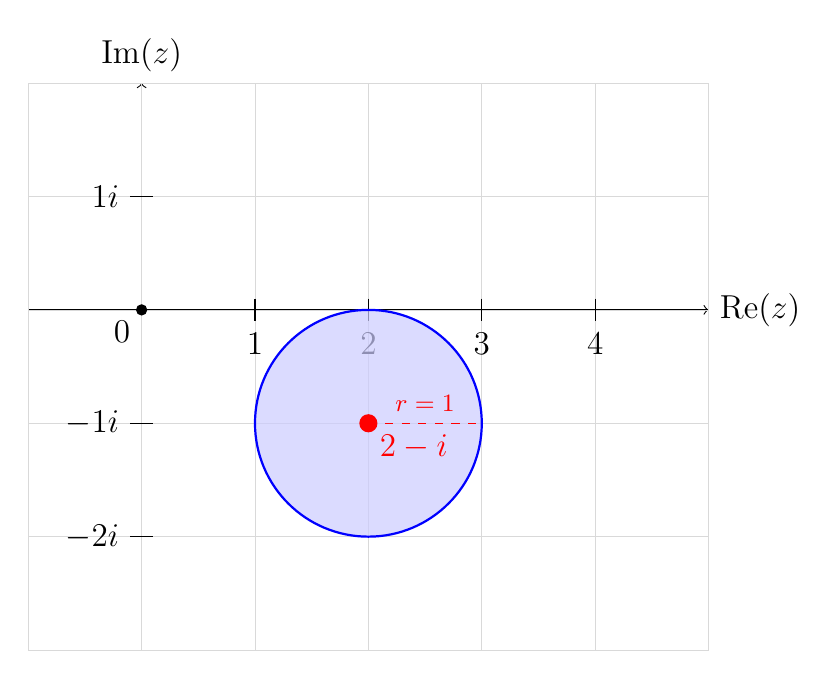
\begin{tikzpicture}[scale=1.2]
    % Draw axes
    \draw[->] (-1,0) -- (5,0) node[right] {$\text{Re}(z)$};
    \draw[->] (0,-3) -- (0,2) node[above] {$\text{Im}(z)$};
    
    % Add grid for better visualization
    \draw[gray!30, very thin] (-1,-3) grid (5,2);
    
    % Mark axis labels
    \foreach \x in {1,2,3,4} {
        \draw (\x,0.1) -- (\x,-0.1) node[below] {$\x$};
    }
    \foreach \y in {-2,-1,1} {
        \draw (0.1,\y) -- (-0.1,\y) node[left] {$\y i$};
    }
    
    % Define center and radius for |z - 2 + i| ≤ 1
    % Note: z - 2 + i = 0 means z = 2 - i, so center is at (2, -1)
    \def\centerx{2}
    \def\centery{-1}
    \def\radius{1}
    
    % Shade the region (closed disk)
    \fill[blue!20, opacity=0.7] (\centerx,\centery) circle (\radius);
    
    % Draw the boundary circle (solid line since it's ≤)
    \draw[thick, blue] (\centerx,\centery) circle (\radius);
    
    % Mark the center point
    \fill[red] (\centerx,\centery) circle (0.08);
    \node[red, below right] at (\centerx,\centery) {$2-i$};
    
    % Add radius indicator
    \draw[dashed, red] (\centerx,\centery) -- (\centerx+\radius,\centery);
    \node[red, above, font=\small] at (\centerx+\radius/2,\centery) {$r=1$};
    
    % Mark origin
    \fill[black] (0,0) circle (0.05);
    \node[below left] at (0,0) {$0$};
\end{tikzpicture}
\end{center}

\begin{itemize}
    \item \textbf{Open:} No, because the boundary is included ($\le$ condition)
    \item \textbf{Connected:} Yes, it's a disk which is connected
    \item \textbf{Domain:} No, because it's not open
    \item \textbf{Bounded:} Yes, all points are within distance 1 from center $(2,-1)$
\end{itemize}

  \item[(b)] $|2z+3| > 4$

  \item[(c)] Im$(z) > 1$

  \item[(d)] Im$(z) = 1$

  \item[(e)] $0 \le \text{arg}(z) \le \frac{\pi}{4}$, where $z \neq 0$

  \item[(f)] $|z - 4| \geq |z|$
\end{enumerate}
\vspace{1cm} % Space for work

\hrule

% Add more problems as needed...
% \newpage
% \section*{Problem 4: [Problem Title]}
% [Problem statement or work space goes here]
% \hrule

\end{document}

%%% Local Variables:
%%% mode: latex
%%% TeX-master: t
%%% End:
